%\documentclass[a4paper,twoside, openodd, final]{memoir}
\documentclass[pdftex,12pt,a4paper]{article}
%\documentclass[defaultstyle,11pt]{thesis}
\usepackage[english]{babel}
\usepackage[top=3.0cm, bottom=3.0cm, left=3.0cm, right=3.0cm]{geometry} %dimenzije strani
\usepackage{hyperref}
\usepackage{longtable}
\usepackage{graphicx}
\usepackage{caption}
\usepackage{verbatim}
\usepackage{color}
\usepackage{tabularx}
\usepackage{multirow}
\usepackage{wrapfig}
\usepackage{fancybox}
\usepackage{framed}
\usepackage{lettrine}
\usepackage{tocloft}
\usepackage{pdfpages}
\usepackage{watermark}
\usepackage[utf8]{inputenc}
\usepackage{comment}
\usepackage{graphicx}
%\usepackage{biblatex}
\graphicspath{ {/Users/lily/lighthouse-taxonomy/sandbox/lily/} }
\usepackage{bibentry}
\nobibliography*

\newcommand{\HRule}{\rule{\linewidth}{0.2mm}}

\usepackage{comment}
 
%\usepackage[
%backend=biber,
%style=alphabetic,
%sorting=ynt
%]{biblatex}
%\addbibresource{proposal.bib}
\bibliography{proposal.bib}
\begin{document}
   \begin{titlepage}
        \begin{center}
%\includegraphics[width=0.15\textwidth]~\\[1cm]

\vfill
\vfill
\textsc{\Large Orthogonal Factorization Solutions in Lighthouse}\\[0.5cm]

\HRule \\[0.4cm]
{ \bfseries A Thesis Proposal \\By Li-Yin Young \\[0.3cm] }



\HRule \\[0.4cm]
{ \bfseries Submitted to the graduate faculty of the \\
Numerical Computation\\
in partial fulfillment of the requirements\\
for the Thesis Proposal and\\
 subsequent MS with Thesis in Computer Science \\[0.4cm] }


\HRule \\[0.4cm]
{\bfseries Elizabeth R. Jessup\\
Boyana Norris\\
Clayton H Lewis \\[0.4cm] }

%\HRule \\[1.5cm]

\vfill
\end{center}
\end{titlepage}

%\documentclass{article}
%\title{Orthogonal Factorization Solutions in Lighthouse}
%\author{Li-Yin Young}
%\date{ }

%\documentclass{article}
\renewcommand*\contentsname{Outline}


%\maketitle
\tableofcontents
\clearpage
\begin{abstract}
Orthogonal factorization are encountered in many fields and there exist different applications for different needs. My work is to add ability to find routines involved in linear least square problems and orthogonal problem to lighthouse. Linear least square problem is generally applied on observational and experimental science. The orthogonal problem in Lighthouse based on the requirement of linear least square problem. The main issues are  challenge is to find finding the right routine and to optimize its implementation. In this thesis I will tackle these issues work on overcoming this challenge by connecting the LAPACK software package with Lighthouse interface such that optimum orthogonal solutions are provided for user?s specific needs. This document explains the research approach, work completed and the proposed work to complete this thesis. 
\vfill
\end{abstract}
\clearpage
\section{Introduction}
\paragraph{}
Orthogonal factorization problems are seen encountered more often frequently than one would might think imagine. We may find see its applications in the scientific fields ranging from Quantum physics [ to Structural engineering [8]. Its widening usage in the increasingly connected internet era is also evident, for example, in search engines (Google Page rank) and social networks.
			
\paragraph{}					
The extensive research in numerical linear algebra has provided given us with different kinds of solutions to least square problems and most of these solutions are optimized depending on the matrix or results we seek sought. Hence, when these various fields encounter eigenvalue problems, we they seek the best solution with respect to a specific set of inputs. As and when the input changes, a different ?best? solution is sought.
\paragraph{}
Orthogonalization can be used to decompose matrices and solve the least square problem. Orthogonal decomposition methods include LQ, QL, RQ, QR, which will be introduced in Section 2.3.
\paragraph{}
One of the challenge for to solve the scientific applications is to lower the time consuming. The These time consuming depends on the size of the problem. Lowering the time-consuming allow us to solve more complicated problem in a shorter time. The size and the complexity of the problem increase influence the cost of processors and their memory. 
\paragraph{}

We apply machine learning tool  to find the best answer and so that we can optimize  the code. 
\paragraph{}

As to the least square problem, orthogonal transformation is a robust type of transformation that can be used to solve the original least square problems and make them easier to compute. Besides solving a general matrix, orthogonal transformation can be used to solve Gauss Markov model problems, which require that one?s data set be normally distributed.\paragraph{}
		
In order to cater to the needs of the increasing demand of solutions to such varied orthogonal problems, a number of free and licensed software packages are made available. These packages cover many different kinds of eigenvalue solutions and somewhere in that pile, lies the solution to that one particular problem, say for example, a structural engineer seeks. 

\subsection{A Statement of Problem} 
\paragraph{}
Using LAPACK functions is a quick way to solve linear algebra questions. LAPACK has too many functions and routines available that could overwhelm a non-expert user. The challenge, therefore, is to select selecting the best solution from the list of available solutions on every new set of inputs and to implement implementing an optimizing optimization on the code. This could be a very taxing procedure for a person not specializing in linear algebra or inexperienced in programming. Thus, unless a person is entirely well versed with eigenvalue problems and coding, deciding and implementing the best solution may take a considerable amount of time and efforts. Therefore, to maintain this convenience, we require a search engine to more easily find the routine that we need.

\subsection{Why orthogonal factorization is important} 
\paragraph{}
We may take a look of the difficulties which we may be confronted with when taking the normal equations approach to solve the least square problem. In least square problem, if A has full column rank, then the nxn symmetric, positive definite system of normal equations 
\begin{equation}
A^{T}Ax=A^{T}b
\end{equation}
has the same solution x as the mxn least square problem Ax ?b. To solve this square system, we compute the Cholesky factorization.[1]
\begin{equation}
A^{T}A=LL^{T}
\end{equation}
where L is lower triangular, and then the solution x can be computed by solving the triangular systems $Ly=A^{T}b$ and $L^{T}x=y$.
  \paragraph{}
We need an alternative way that does not require the formation of the cross-product matrix and the right hand side vector. Orthogonal transformation is a robust type of transformation that is able to make the least square problem easier to compute. For example, orthogonal transformations can be used to solve square linear system without pivoting on numerical stability. This is based on the fact that multiplying a matrix by an orthogonal matrix can transform the matrix in various ways, e.g. rotation or reflection, but still preserve Euclidean length of a vector. Hence, if we multiply both sides of a linear least square problem by an orthogonal matrix, the solution is unchanged. 
We also notice that orthogonal matrices are of great importance in many areas of numerical computation because their norm-preserving property means they do not amplify error. 
\subsection{My contribution} 
\paragraph{}
My contribution is to find the LAPACK routines to solve orthogonal problems. I classify orthogonal problem into two categories. One is the orthogonal decomposition, the other one is the least square problem. I build a decision tree to develop my question flow chart. LAPACK routine is composed by several conditions such as data type, matrix type and factorization type. 
The order of questions matters whether it is straightforward to use our platform to find needed routines. Hence, we need to put the most limited question at the beginning. For example, in the least square problem, LAPACK requires the original matrix should be general matrix and full storage. If the original matrix can?t satisfy this condition, users cannot use LAPACK routine to solve their problem. Therefore, in order to save time to search routines, this question these questions must be put as the in first to ask two questions. 
\paragraph{}
In orthogonal decomposition, one may need to obtain Q matrix. LAPACK routines will return the resault of RQ instead of returning that of Q. Therefore, if one wants to obtain Q, one needs to use additional routines to obtain Q. Therefore, after users choose the type of orthogonal factorization, they need to use corresponding routines to obtain Q matrix. Different types of orthogonal factorization need different routines to help user obtain Q matrix.

\paragraph{}
Since our lighthouse is developed on Django, after building the decision tree for  the question flow chart, I use Django package to finish the orthogonal part which needs to put into lighthouse website. Django provides us with a platform to develop database and webpages. Django also provides a connection between webpages with and  MYSQL. Furthermore, I use MySQL to create a database to save different routines. 


\section{Background}

\subsection{Lighthouse}
\paragraph{}
Lighthouse is an open source web application that provides a search platform to users seeking software solutions to linear algebra problems. It is a search engine designed to help users locate the routine they need in a database of LAPACK, SLEPc and PETSc routines, i.e. functions helpful in solving linear algebra problems. It has a taxonomy of software that is used to provide optimum solutions to matrix algebra computations.
%\graphicspath{ {/Users/lily/lighthouse-taxonomy/sandbox/lily} } 
%\begin{figure}
 %    \includegraphics[scale=0.8]{interface.png}
%\end{figure}
\paragraph{}
A simple guided search in Lighthouse, as shown in figure 1, lets the user select the linear algebra problem he/she wants to solve, which follows a series of simple questions about the input and user preferences. It provides many options for users to specify their conditions, first asking users which questions they seek to solve, and then additional questions pertaining to which types of elements exist in the matrix. The final question will ask users to choose just how precise their answer will be. According to these conditions, system searches the right routines for users. Answering these questions provides the code implementing the routines that best solves user specified problem. This code can be downloaded and used by the user. This application is under development and presently only solutions to linear systems from LAPACK are implemented.

%\graphicspath{ {/Users/lily/lighthouse-taxonomy/sandbox/lily} }
\paragraph{}				
The advanced search option provides questions for someone who is aware of LAPACK terminologies. In each of these cases a user can select the routine for which he/she needs the code to be generated. After obtaining the routines, users can drag the routine to c template and see the source code used to solve linear questions with LAPACK routines. My thesis work will involve providing similar solutions for sparse eigenvalue problems through Lighthouse.
\subsection{Linear Algebra}
The important usages and applications is polynomials and surface fitting. Those fitting problem help us to solve many  problem exist in various field. Therefore, 
\subsubsection{Least Square Problem}
\paragraph{}
Linear Least Squares is a mathematical approach fitting a set of data which minimizes the sum of squared differences between the data values and their corresponding modeled values. It is idealized expressed linearly among unknown parameters in model. Linear least shares take many measurement to smooth out measurement errors or other random variations. It is generally applied on observational and experimental science. For example, astronomers and communications engineers use linear least squares to extract meaningful signals from noisy data. [1]
\subsubsection{Ordinary Linear Least Squares}
\paragraph{}
       For a geometric view of the least square problem[7], we need the notion of orthogonality. QR factorization approach is used to be solved the least square problem. The vector y=Ax span(A) closest to b in Euclidean norm occurs when the residual vector r = b - Ax is orthogonal to span(A). Euclidean norm of r is a the orthogonal projection of b on span(A). We need to find the least squares solution x to make r approximate to 0. Hence, we must have 
\begin{equation}
       0=A^{T}r=A^{T}(b-Ax).
 \end{equation}

\subsubsection{Generalized Least Square Problem}
\paragraph{}
Generalized linear least square model(GLS)[6] extends the Gauss Markov theorem to the case where the error vector has a non-scalar covariance matrix . In statistics, Gauss Markov Model is a regression model to find the trace of a large amount of data. Generalized linear least square model when variance of the observations are heteroscedasticity. In statistics, variables are heteroscedasticity when  each sequence or variance has different variance or each of them has correlation to each other. If one use ordinary least squares to solve the problem, it can be statically sufficient or even given wrong computational results. 

\paragraph{}
\begin{equation}
\min_{(Bx=d)}\left \| Ax-b \right \|
\end{equation}
\paragraph{}
where A and b are $m x n$ and $p x n$ matrices, respectively.The equations Bx=d may be regard as a set of equality constraints on the problem of minimizing the residual\begin{equation}\left \| Ax-b \right \|\end{equation}. The solution only exists if the equations Bx=b are is consistent. Linear equality-constrained least square function equations arise whenever a deterministic relation involving Euclidean-form and the relationship with inner-product and orthogonality is known or postulated. It can be solved directly by Generalized RQ(GRQ) factoirization. Therefore, it allows us to use fewer subroutines to solve problems. 
\paragraph{}
A lgeneralized least square function are mathematically studied from several different perspectives, mostly concerned with their solutions ? the set of functions that satisfy the equation. If a self-contained formula for the solution is not available, the solution may be numerically approximated using computers. 


\subsection{Various Orthogonal Factorization}
\paragraph{}
In this section we introduce various orthogonal factorizations. For this, we first recall the definition of orthogonal matrices.
 Our motivation is to define a type of linear transformation that preserves Euclidean norm. A square matrix Q is said to be orthogonal if its columns are orthogonal to each other and each of them is of the unit length , i.e. if $Q^{T}Q=I$, the identity matrix. (The characteristics of orthogonal matrix tell us that the inverse of an orthogonal matrix is its transpose). Therefore multiplying a vector by Q does not change its Euclidean norm.          

\subsubsection{QR and RQ Factorization}
\paragraph{}
The terminology of generalized QR factorizations refers to the orthogonal transformation that simultaneously transform an $n x m$ matrix A and $n x p$ matrix B to triangular form. [1] Transforming a matrix  to triangular form is accomplished by the QR factorization where Q is an mxm orthogonal matrix and R is an $n x n$ upper triangular matrix. QR decomposition is often used to solve the linear least square problem, and is the basis of a particular eigenvalue algorithm.
\paragraph{}
 RQ method includes solving trapezoidal matrix which is a non-square (or sometimes any) matrix with zeros above (below) the diagonal. 

\subsubsection{LQ and QL  Factorization}
\paragraph{}
LQ and QL are closely related to each other. LQ is the lower-orthogonal-triangular matrix. QL is the orthogonal-lower-triangular factorization. It is well known that the orthogonal facotrs of  a matrix provide information about its row and column space. 
\subsubsection{Singular Value Decomposition (SVD)}
\paragraph{}
If the matrix is singular, it cannot be decomposed by orthogonal factorization directly.   Thus, we use singular value decomposition to decompose a singular matrix. The singular value decomposition(SVD) of an $m x n$ matrix has the form A = UVT, where U is an mxm orthogonal matrix, V is an $n x n$ orthogonal matrix and is an $m x n$ diagonal matrix. [1]
\paragraph{}
Besides solving singular matrix by SVD, LAPACK[2] supplies the routine to solve SVD problem with divide and conquer method. Divide and conquer method divide matrix into sub matrices. Recursively multiplying sub matrices by blocked algorithm. Typically an algorithm that refers to individual elements is replaced by one that operates on subarrays of data. It runs faster but need more work space. [4]%Fix
\subsubsection{Trapozoid Decomposition}
\paragraph{}
In the mathematical discipline of linear algebra, a trapezoidal matrix is a non-square matrix. The number of columns is more than that number of rows.  A non-square matrix is called lower trapezoidal matrix if all the entries above the main diagonal are zero. Similarly, a non-square matrix is called upper trapezoidal matrix if all the entries below the main diagonal are zero. A trapezoidal matrix is one that is either lower trapezoidal or upper trapezoidal matrix. 

 Orthogonal factorization require the original matrix must be nonsingular. If the non-square matrix is to be decomposed by orthogonal factorization, we need to use trapezoidal factorization or singular value decomposition. If the non-square matrix fulfills the requirement of is trapezoidal matrix that, i.e. all the entries below or above are zero, LAPACK routines can help us to orthogonal factorize it by trapezoidal decomposition.

\subsection{Related Work}
\paragraph{}
For some problem LAPACK provides multiple routines to solve. n compared with selecting method to solveUsers pay more attention on obtaining correct answer than selecting methods to solve . Questions designed to ask users should  focus on leading users to find the routines which match their needs. Instead of describing the method for to the  user, the question should focus on the effect of using the routines. 
\paragraph{}
In solving the least square problem, the matrix may be singular matrix. LAPACK, however,  provides the routines to solve the singular matrix. If the matrix is singular, LAPACK provides two different routines to solve. One routine uses QR factorization with column pivoting; the other one uses SVD to solve.  There is a paper \textit{"Stable And Efficient Spectral Divide and Conquer Algorithms for the Symmetric Eigenvalue Decomposition and the SVD"}[4] evaluate the performance between QR with column pivoting and Gaussian Elimination with column pivoting. 
[1] QR with column pivoting is faster than the Gaussian Elimination with column pivoting since it leads to faster SVD. However, it needs more memory space. In addition, in orthogonal decomposition, some routine runs faster but users cannot obtain an orthogonal matrix solely after implementing the routine. These information should be listed in our questions. 
\section{Research Approach}
\paragraph{}
LAPACK routines are distinguished by data types, matrix types, precision types, and element types stored in matrices. Currently to find the best fits solutions for a least square problem can be solved by  looking up common search engines or technical manual of the available software package.When using search engines, one need to make an  effort to specify their need precisely. Without the help of search engine, a  user may have to go through technical manuals and find the subroutines to compose the routine. Both works require a user have best understanding of linear algebra. 

\paragraph{}
The main aim of this research is to provide optimum solutions to user specific orthogonal problems through the Lighthouse interface. This search engine needs to have a user-friendly interface. In this case, the solution does not just mean to provide providing the best orthogonal solver but also to generate generating the complete code that can be downloaded by the user and used for its their application. To achieve this goal we may can divide this problem into three sub-problems: 	
\begin{enumerate}
\item \textbf{Questions}: We design questions which lead a user to find routines step by step  without spending time on understand the background of linear algebra and technical manuals. The content and order of these questions must be comprehensive enough to lead to a narrowed list of solutions. It must concise enough so that the user  can accessible to understand instead of abandoning the entire process during answering questions. Additionally, the order of question also affects matter the efficiency to search routines. Some routines only allow to be composed by specific subroutine; if the matrix?s condition does not match, it can not be solved. 
\item \textbf{Solutions}: There is a wide variety of solutions for different kinds of orthogonal problems depending on the type of matrix, the application of the least square problem and so on. The choice of the kind of orthogonal decomposition depends on the type of the least square questions. This task involves narrowing down to the most apt orthogonal solver, depending on the answers to questions posed in the first task. In addition, some subroutines provide routines to run more faster but requiring more memory space. The information should be listed in our question. 
\item \textbf{Implementation}: The final task is to implement the code and plug it into the Lighthouse interface. This code should support all the selections made by the user in the Questions section. Some answer may need to implement more than one routine. In orthogonal decomposition, LAPACK routines only return the result of QR. If the user needs to obtain Q matrix, a user needs to use additional routine. The implementation part also includes updating the Lighthouse interface with the questions and delivering an appropriate solution in the form of generated code after users selection.
\end{enumerate}
\paragraph{}
All the three tasks mentioned above are clearly interdependent. When we find an orthogonal factorization solution least square problem solution which works best for a specific matrix attribute, we might need to update the question list to get that attribute information from the user. If we add more questions, we need to make sure that there is a change in the proposed solution depending on the answers. Although the questions save user?s effort to look at manuals, if the questions layers are too many, user would lost patient to find routine by our searching interface. 
Similarly, in order to reach a decision on the solution we need to run some experiments with sample inputs, and hence, we need to implement the code alongside. The questions may also need to be updated depending on the results. Thus, we cannot take an approach of tackling one sub-problem at a time. 


\section {Development Process}
\paragraph{}
The first step, therefore, was to obtain a good understanding of the LAPACK package. LAPACK, which stands for Linear Algebra Package which itself provides a powerful set of tools and base data structures for numerical problems on high performance computers. LAPACK can be considered as an extension of LINPACK which makes use of certain tools and data structures available in LINPACK to provide efficient solutions for eigenvalue problems. 
\paragraph{}			
LAPACK were installed in a Linux(Ubuntu) operating system in order to run a few examples and to get some understanding of LAPACK programs.
\paragraph{}					
Next, The important usage of orthogonal matrix is to solve the least square problem. Therefore the requirement of solutions to orthogonal problems depends on the need of least square problem. Orthogonal decomposition and least square problem  were studied keeping in mind the implementation in LAPACK.
\paragraph{}
The least square problem orthogonal routines provided by LAPACK supports real as well as complex problems. Some of the external packages do not support complex problems. LAPACK  supports generalized and standardized orthogonal factorizations solutions. Properties of each of the orthogonal  and least square problem solvers in LAPACK were studied. A brief description [13] of some of the solvers and properties will be given below. 

\subsection{Package Used}

\textbf{LAPACK}
\paragraph{}
LAPACK [2] is an acronym for Linear Algebra Package. As the name indicates, LAPACK contains subprograms for basic operations on vectors and matrices. [2] LAPACK subroutines are designed to be used for exploiting BLAS as much as possible.  Like the BLAS routines, the LAPACK routines are virtually self-explanatory. The calling sequences are standardized so that programs that call BLAS will work on any computer that has BLAS installed. The source code for LAPACK is available through Netlib. If one has a fast version of LAPACK, one will  get high performance on all programs that use LAPACK. Hence LAPACK provides a simple and portable way to achieve high performance for calculations involving linear algebra. 
LAPACK subroutines are a de facto standard software library for numerical linear algebra. LAPACK specifies a set of low-level subroutines that perform common linear algebra operations such as solving system of simultaneous equations, least square equation, eigenvalue problem and singular value decomposition. LAPACK also  includes routines to implement the associated matrix factorizations such as LU, QR, Cholesky and Schur decomposition. 
Several LAPACK library implementations have been tuned for running on the then-modern vector computer architectures with shared memory. Highly optimized implementations have been developed by hardware vendors such as Intel and AMD. \\
\\
\textbf{Django}
\paragraph{}
After finishing outlining the questions and the experiments of different matrix sizes, I use the Django to develop web pages and the connection to the database. Django is a free and open source web application, written in Python. The important application for of Django is to develop database-driven website. Django help us ease the difficulties of making the connection between website and database. Django provides an optional administration  to create, read and delete interface. The core of Django is a MVC framework[3] consisting with an object-orientational mapper which mediates between data models and a relational database. Django can translate HTML forms and into values suitable for to MVC frame work which is is  a software architiectural pattern for implementing users interface. MVC divides software application into controllers, models and views. Controller sends commands to ask models to change states(i.e. editing documents). Models notify the views to produce the updated output. A view is used to generate an output representation to for the user.    

\subsection{Requirements and specifications}
\subsubsection{Search Capability and User Interface design}
\paragraph{}
Lighthouse provides three different graphical user interfaces to help users of different back- grounds to use the numerical software. 
The question flow chart outlines the steps a user must follow to find the desired routine. The Lighthouse website already has a search engine for other linear problems, such as eigenvalue and singular value decomposition. Each interface offers the code generation service and tuning tools included in the taxonomy. The following subsections discuss more on the components of the Lighthouse user interfaces. 

\paragraph{}
After the user chooses what they want to compute, Lighthouse generates more detailed questions, where three questions have been answered and the next question is being asked. Once the user has answered all the questions, Lighthouse returns a single routine in the search result area of the interface.
\paragraph{}					
The user who has already learned how to utilize Lighthouse will have an easier time with orthogonal factorization if the search engines for all linear problems look the same. Therefore, to organize orthogonal factorization question flow chart, the order of questions need to be the same with as the question order for other linear problems.  The order of  question matters whether it is straightforward to use our platform to find needed routine. Hence, we need to put the most limited question at the beginning. For example, in the least square problem, LAPACK require original matrix should be general matrix and full storage. If the original matrix cannot satisfy this condition, user cannot use LAPACK routine to solve their problem. Therefore, in order to save time to search routines, these questions must put as in the first two to ask. 
\\
\\
\textbf{Problem type? (Least Square Problem, Orthogonal Decomposition) }
\\
\\
\textbf{Least Square Problem}
\begin{itemize}
\item Rank efficient or inefficient?
\item Complex or Real?
\item Full storage ?
\item General Matrix?
\item linear constrained-equally  least square matrix or Generalize linear least square problem?
\end{itemize}
\textbf{Orthogonal Decomposition}
\begin{itemize}
\item General or trapezoidal matrix?
\item Rank efficient or inefficient?
\item Complex or Real?
\item Singular matrix?
\end{itemize}
\paragraph{}
The first question need to ask is whether the matrix A is rank efficient or deficient. If A has linearly dependent columns, the QR factorizations still exists, but the upper triangular factor R is singular. Thus, many vectors x will give the same minimum residual norm. The least square solutions therefore cannot be unique. 
\paragraph{}
If the matrix is singular, it needs to be computed by RQ factorizations with column pivoting or singular value decomposition.  Users can choose which method they want to solve singular matrix. After knowing whether A is singular or nonsingular, the second layer will ask users whether A contains any complex number. 
\graphicspath{ {/Users/lily/lighthouse-taxonomy/sandbox/lily} }
\begin{figure}
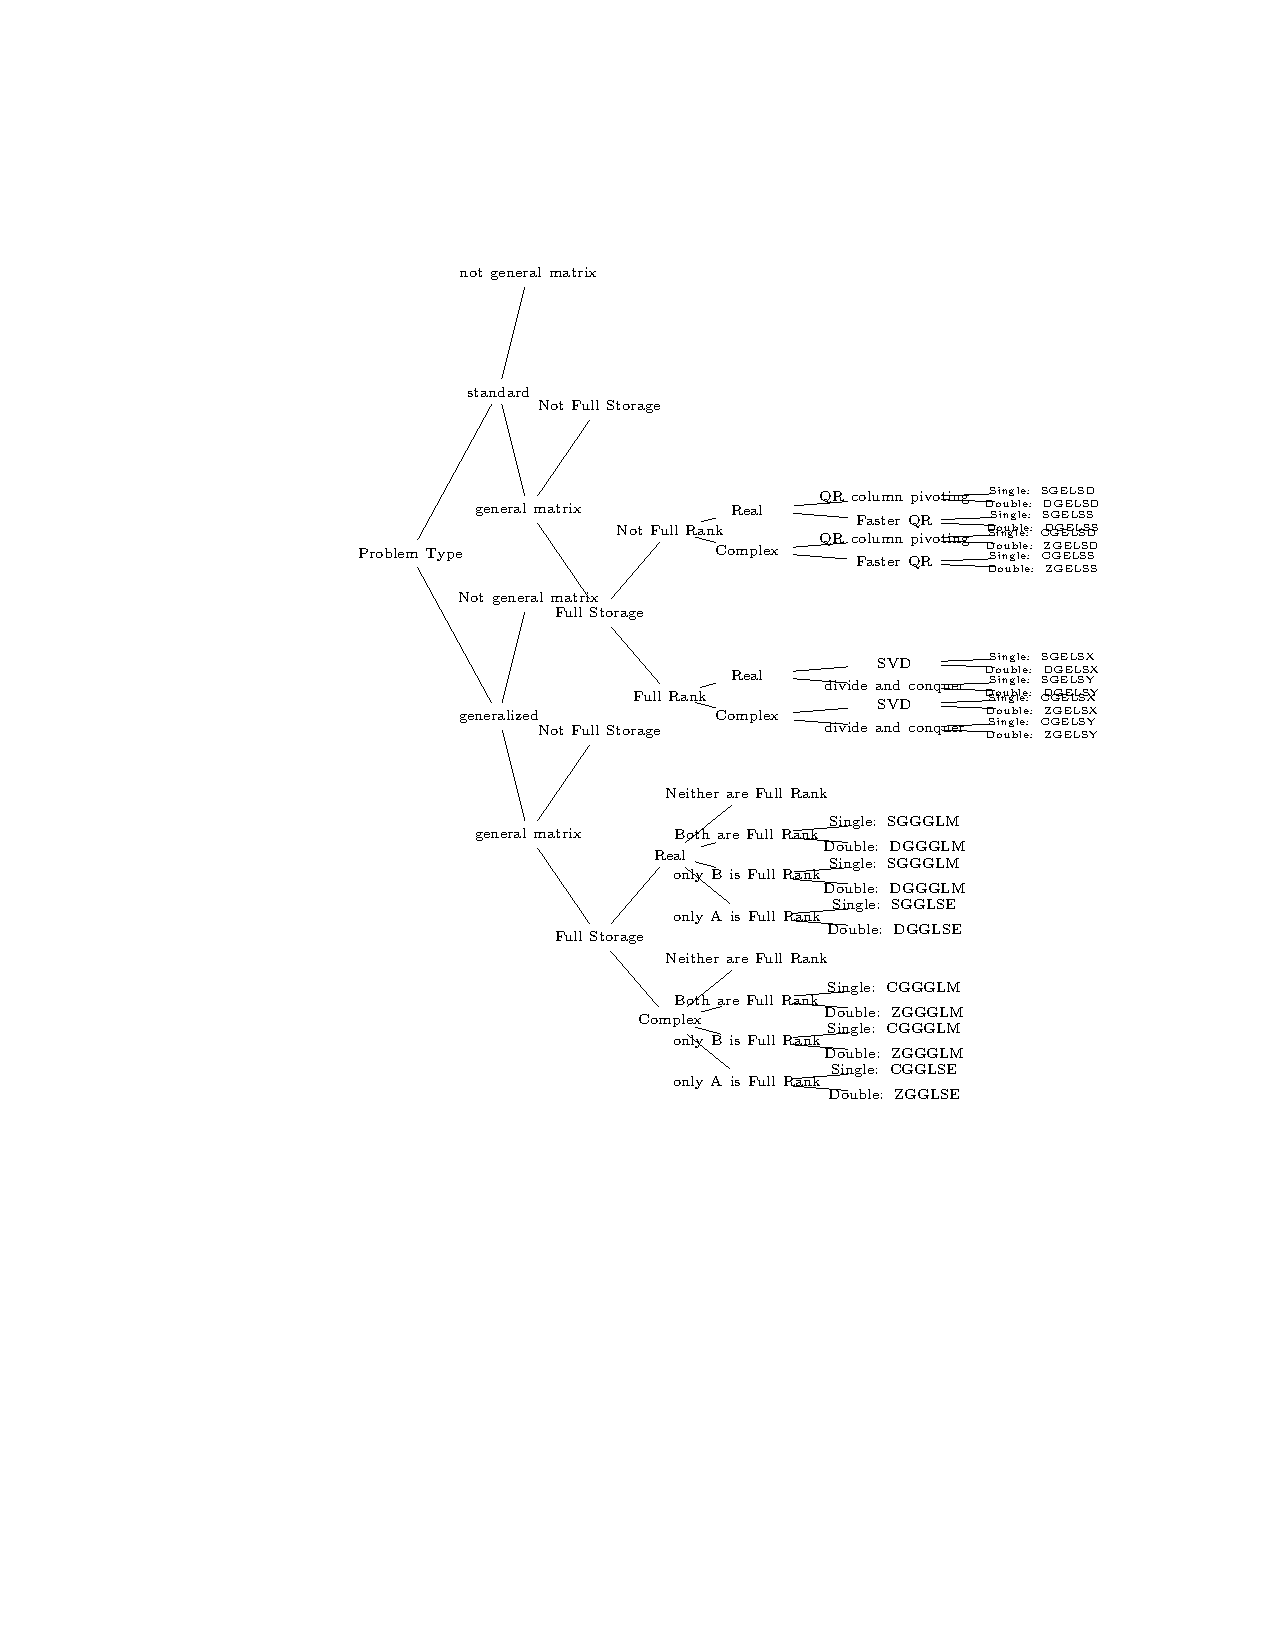
\includegraphics[scale=0.8]{vcl_decisionTree.pdf}
\caption{ Decision Tree for Linear Square Problem} 
\end{figure}
\subsubsection{Orthogonal routines for linear equation}

\paragraph{}
Orthogonal vectors are a special set of orthogonal unit vectors which have a common characteristic: a matrix composed of orthogonal vectors, if transposed, is equal to its inverse.  The decomposition of a square matrix A into an orthogonal matrix and a triangular matrix is known as orthogonal decomposition. 
\paragraph{}
In linear algebra, the orthogonal matrix is a square matrix with rows and columns that are orthogonal unit vectors.  The orthogonal matrix has the property that, when it is multiplied by itself, it results in the identity matrix. We can use this characteristic to solve least square question. In order to solve the least square equation we multiply orthogonal vectors to the coefficients on each side, with our question matrix being the identity matrix. In order to solve a least square question, LAPACK will transform the question matrix by way of QR decomposition. In order to obtain Q from QR, we need to use -mqr routine. Then we can multiple the right side by Q to solve for x. 

\section{Purposed work}
\paragraph{}
To avoid spending time on searching for the routines needed to solve their problem, as well as to make sure that users use the correct routines to solve their problem, it is necessary to build a search engine to help users find the correct routines. This thesis proposes to solve the problem stated above by providing a convenient interface such that the a user can make selections to specify his/her input and then the subsequent application then finds the best solution. After obtaining the routines, a user can generates codes for the specific problem and then download and use it via lighthouse interface. Such an application would makes complicated solutions much more accessible. A user can hence, spend time on the actual scientific computation problem rather than trying to find and implement an optimum solver. 

\paragraph{}
Continuing on the description in previous section, the implementation and properties of the orthogonal solvers in the external packages will be studied. The list of questions will be updated accordingly.\\
\\
\textbf{Experiments with different matrices}\\

\paragraph{}
Next, some experiments will be run for different permutations of answers to these questions so as to further narrow down the solver. For this, LAPACK provides routines to solve matrices with different properties. One uses these properties to test different orthogonal solvers. The table below shows the various attribute options that can be used for each of the orthogonal solvers provided in LAPACK. 
\begin{center}
\begin{tabular}{|p{1.5cm}||p{1.5cm}|p{1.5cm}|p{1.5cm}|p{1.5cm}|p{1.5cm}|p{1.5cm}|}
 %\caption{Various Inputs Parameters}
\hline
\multicolumn{7}{| c |}{Least Square Problem}\\
\hline
 Examined Parameters:&Problem type & Rank efficient & Complex or Real & Full storage & General Matrix & Linear Square Problem Type\\
\hline
\end{tabular}
\end{center}

\begin{center}
\begin{tabular}{|p{1.5cm}||p{1.5cm}|p{1.5cm}|p{1.5cm}|p{1.5cm}|}
 %\caption{Various Inputs Parameters}
\hline
\multicolumn{5}{| c |}{Orthogonal Decomposition}\\
\hline
 Examined Parameters:&Problem type &General or trapezoidal matrix& Rank efficient & Complex or Real \\
\hline
\end{tabular}
\end{center}

 \paragraph{}
For some kind of solutions of the least square problem, LAPACK will supply multiple routines. The  performance depends on the matrix size and the number of times of iteration.To help users to find the probable routine,  we evaluate the results based on the tolerance and the number of times of iteration. We also put a counter in iteration loop so that we can obtain the average time for each loop. For solvers that come close to each other in performance, we can increase the matrix size to escalate the difference of performance. To make the comparision more clear, one can plot it against the number of iterations. A study of this trend will give us an idea of which orthogonal solver works best as the size of matrix increases. This will help us in providing better suggestions to the user.\\
\\
\textbf{Plugging into Lighthouse}

\paragraph{}
After obtaining the answers to every attribute selections and optimizing results, all that is left to do is updating the Lighthouse interface with solutions to orthogonal problems. This task requires adding the questions and the information help user to make decision. Some of questions influence subsequent questions which needs updating after selection. Some routine only allow specific subroutine. Hence, a short listing the recommended notification come along with orthogonal solver on the right. When a user finishes answering all questions, the corresponding code (in C and Fortran) and script file will be generated and the user will be able to download it. \\
\\
\textbf{Testing}
\paragraph{}
Test the added functionality to lighthouse by asking users to perform some test cases. In cognitive science, there is a method called thinking aloud. The experiment require user to say what they are thinking about during the test. We can require user to tell us what they think about while they are using the added functionality in Lighthouse. The report help us find out what difficulities user would meet when using Lighthouse search engine to look for orthogonal routine. 

\section{Conclusion}
\paragraph{}
In this chapter we present our conclusions about the method we developed for enabling Lighthouse to provide the users use LAPACK routines and helpful suggestions about which routines they should use if there are multiple usage routines can solve same problem. 
\paragraph{}
Lighthouse have functionality to that allows users to download programs with LAPACK routine for solving linear systems using an interactive web user interface. In addition, we developed a technique that enables Lighthouse to take in a matrix from a user, analyze it and recommend them which method can give them the fastest solution. A user-friendly application that provides a platform to search for the solution and generates code with hassle free usage would immensely help solution seekers. 
\paragraph{}

\bibliographystyle{alpha}
\bibliography{proposal.bib}

\Large\textbf{Bibliography}
\paragraph{}
\small{[1] Scientific computing: An Introduction Survey,Michael T. Heath, MC-graw Hill, 2002}
\paragraph{}
\small{[2] Jiawei Han, Micheline Kamber, and Jian Pei, Data mining concepts and techniques, Morgan Kaufmann Publishers, Waltham, Mass, 2012}
\paragraph{}
\small{[3] Donald Knuth, Quantum Physics, $http://en.wikipedia.org/wiki/Quantum_physics$}
\paragraph{}
\small{[4] Yuji nakatsukasa and nicholas j. Higham, stable and efficient spectral divide and conquer algorithms for the symmetric eigenvalue
Decomposition and the svd, siam j. Sci. Comput}
\paragraph{}
\small{[5]  Aitken, On Least-squares and Linear Combinations of Observations,  Proceedings of the Royal Society of Edinburgh 55: 42?48, 1934}
\paragraph{}
\small{[6] Barlow, Jesse L., "Chapter 9: Numerical aspects of Solving Linear Least Squares Problems", in Rao, C.R., Computational Statistics, Handbook of Statistics 9, North-Holland, 1993} 
\paragraph{}
\small{[7] E. Anderson, Z. Bai, C. Bischof, J. Demmel, J. Dongarra, J. D. Croz, A. Greenbaum, S. Ham- marling, A. McKenney, S. Ostrouchov, and D. Sorensen, LAPACK Users' Guide, Society for Industrial and Applied Mathematics, 1999}
\paragraph{}
\small{[8] Donald Knuth, Quantum Physics, $http://en.wikipedia.org/wiki/Quantum_physics$}
\end{document}

%\medskip
%\printbibliography[heading=bibintoc,title={Bibliography}]
%\clearpage
%\printbibliography[heading=subbibintoc,type=article,title={Articles only}]
%\printbibliography[type=book,title={Books only}]
%\printbibliography[type=online,title={Online only}]













